\newpage
\section{\emph{SMALL MODULAR REACTORS (SMRs)}} \label{small_modular_reactors}

Los reactores modulares pequeños, más conocidos como \acrfullpl{smr}, son \textbf{reactores nucleares avanzados que producen entre 10 y 300 MWe por módulo} (\cite{nea_smrs_2021}). Aunque se trata de una potencia considerablemente menor a la de los reactores nucleares convencionales de alta potencia ---que suele ser de más de 1.000 MWe---, es precisamente esta característica la que los hace muy atractivos, dadas las múltiples ventajas que esto proporciona en cuanto a versatilidad y variedad de aplicaciones.

Actualmente, hay un creciente interés por esta innovadora tecnología. Durante la \emph{Conferencia Internacional sobre el Cambio Climático y el Papel de la Energía Nuclear} celebrada en septiembre de 2019, muchos Estados Miembros consideraron a los \acrshortpl{smr} como ``una opción nuclear potencialmente viable para contribuir a mitigar el cambio climático'' (\cite{oiea_informe_2019}). A raíz de esta conferencia, en abril de 2021, el \acrfull{oiea} creó la \emph{Plataforma sobre Reactores Modulares Pequeños y sus Aplicaciones (Plataforma SMR)}, un mecanismo que coordina las actividades del \acrshort{oiea} en este campo y proporciona un punto de encuentro común para los Estados Miembros y otras partes interesadas. Por último, cabe destacar que la Comisión Europea creó el pasado 6 de febrero de 2024 una alianza con el objetivo de facilitar y acelerar el desarrollo y el despliegue de los primeros proyectos de \acrshortpl{smr} en Europa a principios de la década de 2030: la \emph{Alianza Europea Industrial en SMRs}. Todo esto refleja una apuesta creciente por los pequeños reactores modulares que debe ir acompañada por un fuerte impulso en el \acrshort{idi} en este ámbito.

\subsection{Breve recorrido histórico: Orígenes y desarrollo}

El origen de los \acrshortpl{smr} es militar y se remonta a los años 50, cuando se diseñaron por primera vez los pequeños reactores que se emplearon para la propulsión naval de submarinos nucleares, portaviones y rompehielos. Con la elaboración del primer subarino nuclear, el \emph{Nautilus}, diseñado por la armada estadounidense y puesto en marcha en enero de 1955, se puso de manifiesto las importantes ventajas que esta tecnología ofrecía a los grandes navíos militares: posibilidad de inmersión por tiempo ilimitado ---en el caso de los submarinos--- al no requerir oxígeno para su funcionamiento, alto nivel de disponibilidad y de independencia de abastecimiento de combustible, elevada versatilidad y mayores velocidades de desplazamiento (\cite{propulsion_naval_nuclear}).

\begin{figure}[h]
    \centering
    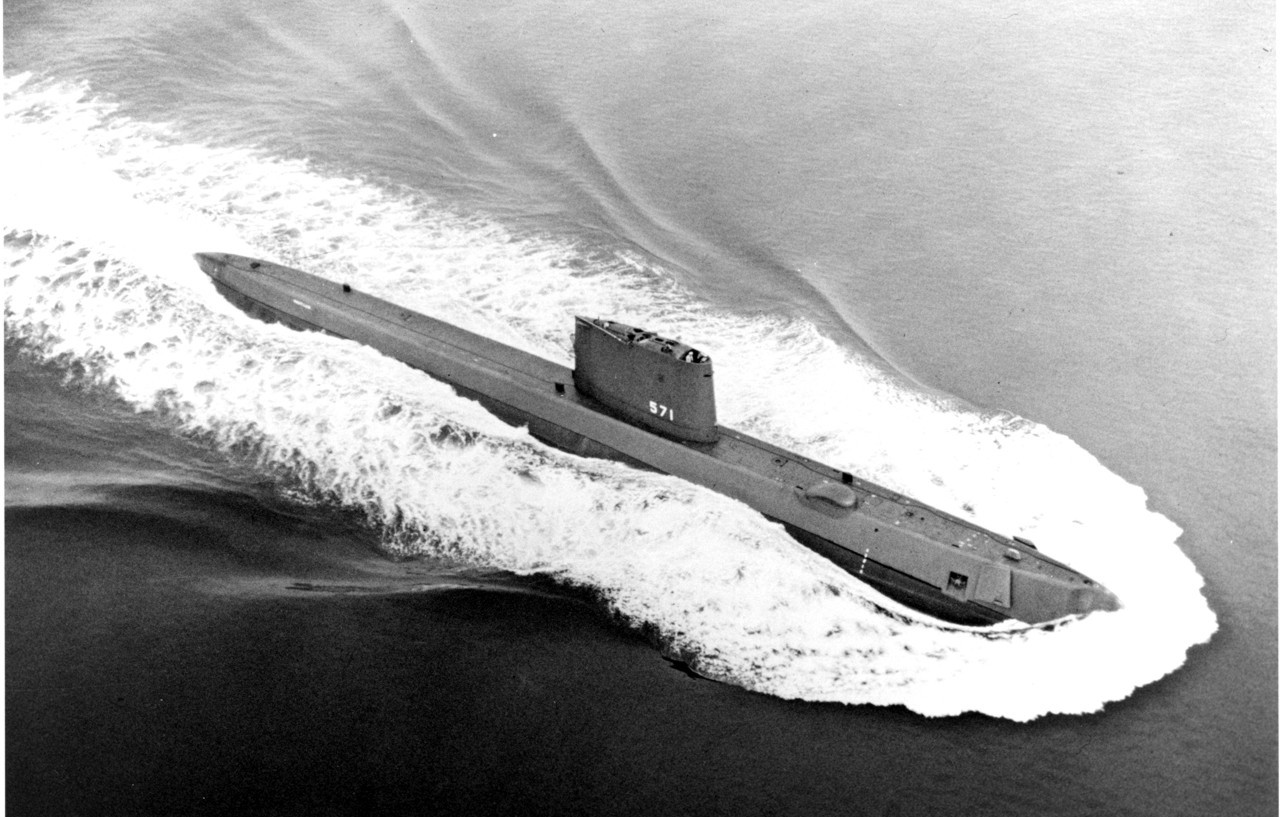
\includegraphics[width=0.55\textwidth]{content/figures/nautilus.jpg}
    \caption{\emph{USS Nautilus (SSN-571)} en alta mar con su reactor S2W de 10 MW de Westinghouse (\cite{poder_naval}).}
    \label{fig:nautilus}
\end{figure}

No fue, sin embargo, hasta más adelante cuando empezaron a desarrollarse los pequeños reactores nucleares comerciales para uso civil. El primer prototipo fue diseñado en 2007 por un equipo de científicos estadounidenses de la \emph{Oregon State University (OSU)} y se le llamó \emph{Multi-Application Small Light Water Reactor (MASLWR)}. Con una potencia de 45 MWe, el MASLWR, fue el prototipo con el que empezó a trabajar la empresa \emph{NuScale Power}, la cual consiguió lanzar en 2022 al mercado estadounidense el primer \acrshort{smr} apto para operar.

Hoy en día \textbf{existen en todo el mundo más de 80 diseños y conceptos de \acrshort{smr}} en diversas etapas de desarrollo, cuatro de los cuales se encuentran en etapas avanzadas de construcción en Argentina, China y Rusia.

\subsection{Características generales}

Los diseños de \acrshortpl{smr} están progresando rápidamente, partiendo del objetivo de integrar sistemas para conseguir modulizar los reactores al mismo tiempo que se introducen mejoras significativas para el funcionamiento eficaz y seguro de los mismos. De esta manera, se están desarrollando prototipos con muy buenas prestaciones en lo que a seguridad, flexibilidad, costes, gestión de residuos y variedad de aplicaciones se refiere.

\subsubsection{Seguridad}

Debido a la experiencia de más de 60 años de operación de las centrales nucleares, se han llevado a cabo gradualmente grandes mejoras de seguridad y control de las mismas. Los reactores nucleares avanzados que se están desarrollando en los últimos años, incluidos los \acrshortpl{smr}, incorporan estos avances tecnológicos. Entre las múltiples mejoras incorporadas, cabe destacar el empleo de innovadores \textbf{sistemas de seguridad pasiva}. Los sistemas pasivos son aquellos que no requieren de la acción de un operador o de realimentación electrónica para funcionar, sino que su actuación se asegura por principios físicos independientes de energía externa. Son, por tanto, especialmente útiles en casos de emergencia en los que, aunque se perdiera el suministro eléctrico de la central, los sistemas de seguridad deberían funcionar sin ningún problema (\cite{glosario_seguridad_oiea}). Algunos ejemplos de este tipo de sistemas son los recombinadores autocatalíticos pasivos\footnote{Eliminan los posibles gases combustibles generados dentro de la contención en accidentes severos mediante la recombinación o combustión de una manera gradual, minimizando así el riesgo de una explosión de hidrógeno.}, el \acrfull{svfc}\footnote{Posibilita la despresurización controlada del Edificio de Contención en caso de fusión del núcleo y la reducción de la cantidad de material radiactivo que podría ser liberado al exterior.} o el sistema de sellado pasivo de las bombas del circuito primario\footnote{Permite reducir significativamente o, incluso, eliminar la fuga de refrigerante a través de los sellos sin requerir operación manual. Se activan por temperatura y bloquean automáticamente
el paso de agua.}. Todos estos nuevos sistemas se han ido implementando en las centrales nucleares actualmente en operación y se han incorporado, junto con muchos otros avances, en los diseños de los reactores avanzados.

En el caso de los \acrshortpl{smr}, la mayor dependencia de los mecanismos de seguridad pasiva, al reducir la necesidad de sistemas activos ---como las bombas de refrigeración del reactor---, simplifica las evaluaciones de seguridad y reduce las posibilidades de fallo de la instalación. La menor potencia de salida y la mayor relación superficie-volumen ofrecida por núcleos más pequeños aumentan la eficiencia de los sistemas de seguridad pasiva tanto para condiciones de operación normales como para transitorios indeseados. Por ejemplo, muchos diseños de tipo \acrshortpl{lwr} disponen de grandes depósitos de agua para enfriar pasivamente los sistemas de reactor incluso en circunstancias extremas (por ejemplo, en caso de pérdida de suministro eléctrico exterior). Una mayor dependencia de los sistemas de enfriamiento pasivo permite \textbf{diseños más simplificados y una operación y mantenimiento más eficientes}. 

Por otro lado, su \textbf{diseño integral} incorpora todos los componentes del sistema de suministro de vapor nuclear (del inglés, \acrshort{nsss})\footnote{Incluye los principales sistemas y componentes de una central nuclear: todo el sistema del refrigerante del reactor (el circuito primario), los sistemas fluidos auxiliares y los principales sistemas eléctricos, de instrumentación y control requeridos para la operación de la planta.} en un solo recipiente. Consecuentemente, la mayor relación superfície-volumen de estos reactores mejora la disipación del calor residual. Esto implica que la cantidad de refrigerante contenido en la vasija del reactor es considerablemente mayor que en las configuraciones tradicionales de bucle externo, lo cual aumenta la capacidad calorífica\footnote{Cantidad de energía necesaria para aumentar la temperatura de un sistema en una unidad de temperatura.} y la inercia térmica\footnote{Capacidad que tiene un sistema de almacenar calor. Es directamente proporcional a la capacidad calorífica, por lo que a mayor inercia térmica, mayor cantidad de energía se requiere para elevar la temperatura de un cuerpo.} del sistema. Además, para la extracción del calor residual se han desarrollado nuevas metodologías, como apoyar la refrigeración convencional con la convección natural de aire.

\begin{figure}[h]
  \centering
  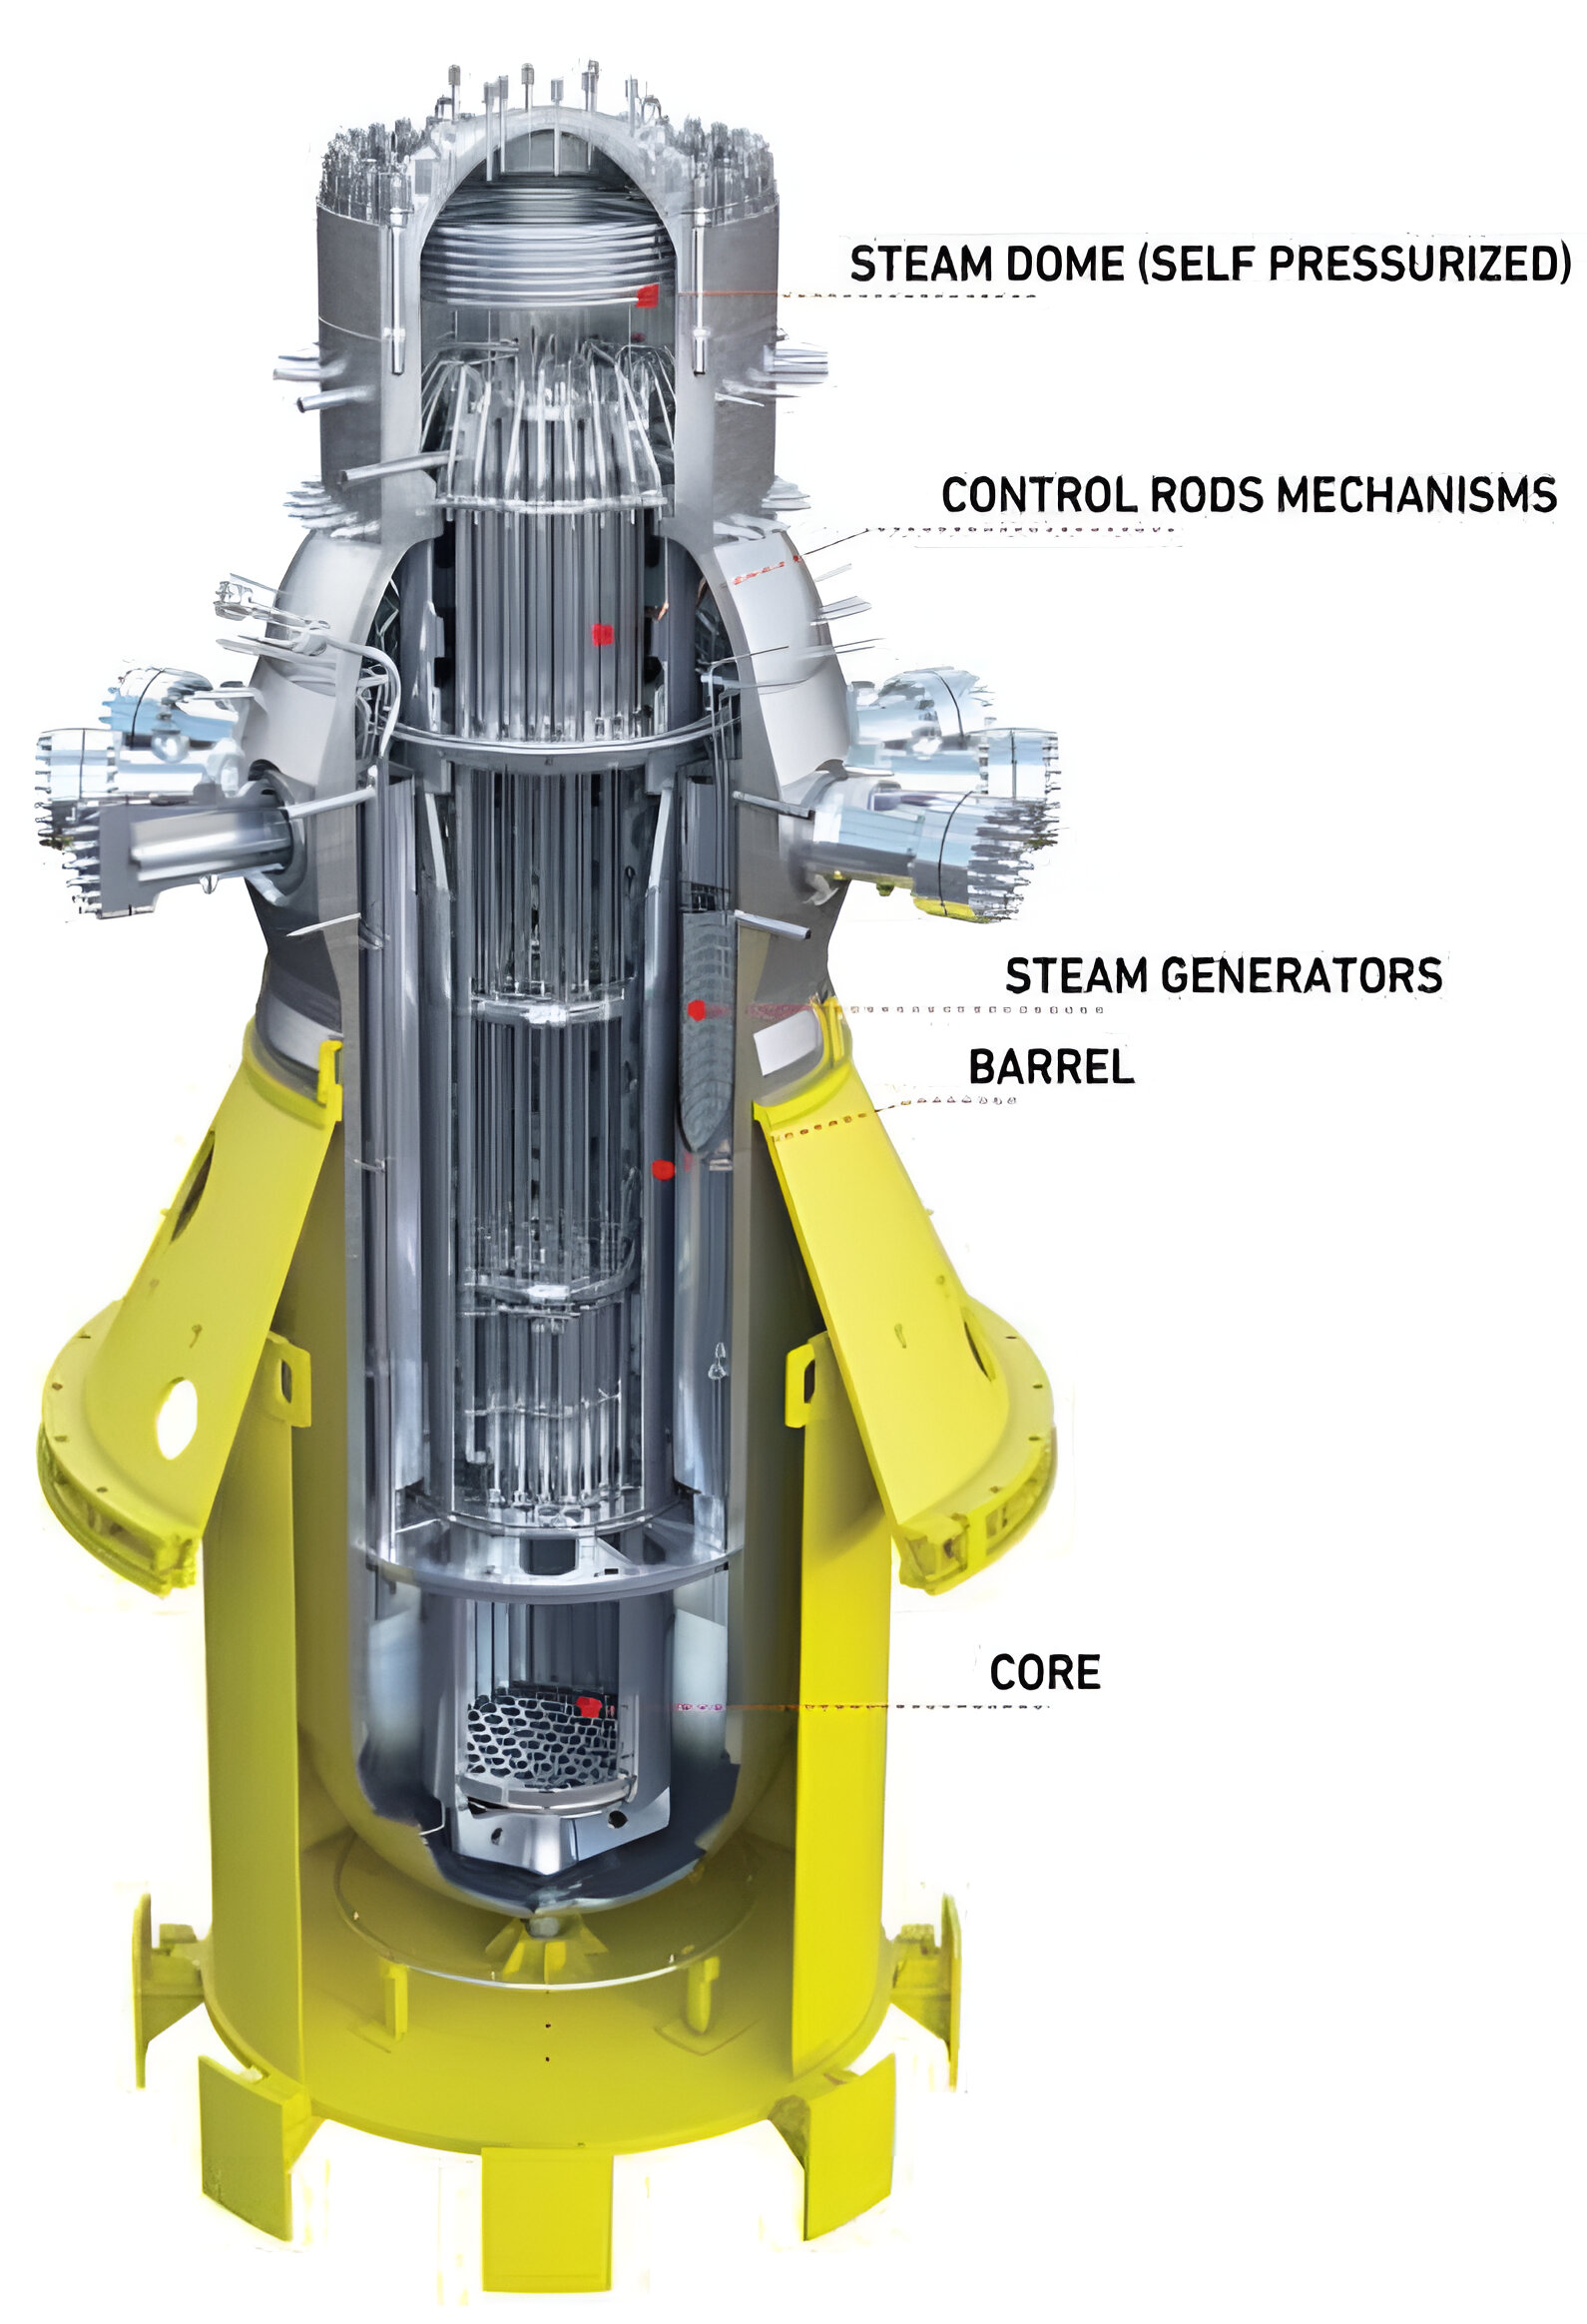
\includegraphics[width=0.62\textwidth]{content/figures/carem.jpeg}
  \caption{Vasija del reactor CAREM (ver tabla \ref{tab:smrs_agua_tierra}) que alberga de forma integral los componentes del \acrshort{nsss}: el núcleo, los generadores de vapor, el refrigerante primario, etc. junto con otros elementos fundamentales, como las barras de control (\cite{iaea_smr_booklet_2022}).}
  \label{fig:carem}
\end{figure}

La compacta configuración de los \acrshortpl{smr} \textbf{reduce la probabilidad de accidentes y la gravedad de los mismos}. Por ejemplo, un diseño más compacto reduce considerablemente el número de penetraciones en la vasija de reactor para la instalación de tubos, lo cual se traduce en una disminución del número de puntos con probabilidad de fuga, haciendo así más resistente al reactor frente a un accidente de pérdida de refrigerante (del inglés, \acrshort{loca}). Otro ejemplo es que la integración de las barras de control dentro de la vasija del reactor elimina el riesgo de accidentes por eyección de las mismas, suceso que puede ocurrir en un reactor convencional y que provoca un súbito incremento de reactividad y, por tanto, un aumento incontrolado de la potencia del reactor. Cabe mencionar, por último, que al trabajar con mayor inercia térmica y menor densidad de potencia\footnote{Cantidad de potencia generada por unidad de volumen. En los \acrshortpl{smr}, al ser mucho menor la potencia generada, la potencia densidad específica es baja.}, la respuesta frente a transitorios de temperatura es más lenta, lo cual aumenta los márgenes de seguridad y ralentiza el posible descontrol del reactor en situaciones adversas.

Además, la reducción del inventario del núcleo del reactor hace que se requiera \textbf{menos blindaje} para la protección del mismo y que las dosis de exposición de los trabajadores sean menores. Tal y como se ha comentado en el párrafo anterior, el hecho de tener un núcleo más pequeño reduce la probabilidad de accidente e implica menor energía en la posible expulsión de emisiones radiactivas. De esta manera, \textbf{se reduce la extensión necesaria de las zonas de planificación de emergencia (\acrshortpl{epz})}\footnote{Zonas que rodean a la central nuclear que se proveen, en base al plan de emergencia correspondiente, de las necesarias medidas de protección de cara a un posible accidente}. Esto último implica que estas plantas podrían ubicarse más cerca de los consumidores finales, ofreciendo un servicio más directo y reduciendo los problemas derivados del transporte de electricidad a grandes distancias.

Por último, las características de los \acrshortpl{smr} hacen posible su \textbf{ubicación subterránea}, que proporciona una mayor protección frente a posibles peligros naturales ---terremotos, inundaciones, huracanes, etc.--- o provocados por el ser humano ---como podría ser el impacto de un avión---. Múltiples diseños desarrollados en los últimos años, como el que se muestra en la figura \ref{fig:ultra_safe_nuclear_mmr}, están optando por ubicar de esta manera los principales componentes de la planta (\cite{nea_smrs_2021}).

\begin{figure}[h]
  \centering
  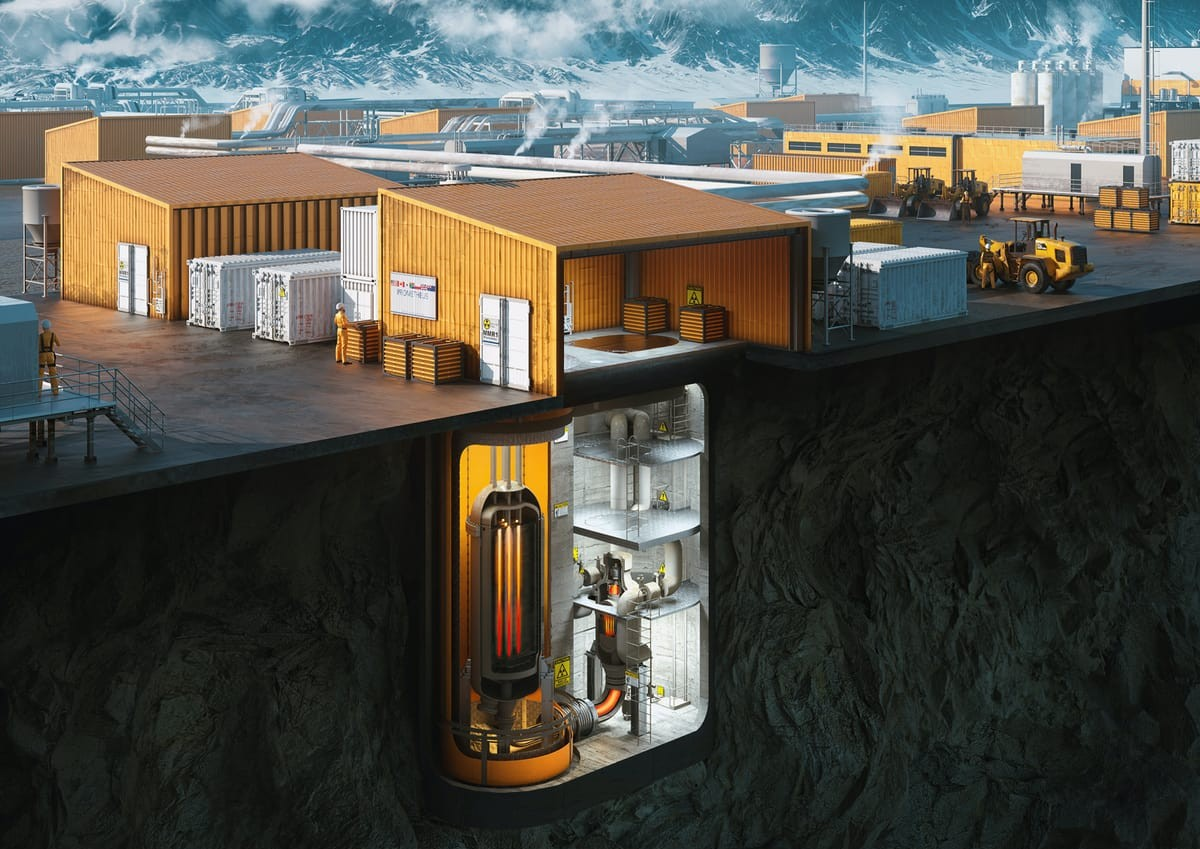
\includegraphics[width=0.65\textwidth]{content/figures/ultra_safe_nuclear_mmr.jpg}
  \caption{\emph{\acrshort{mmr} Energy System} de entre 3,5 y 15 MWe de potencia, diseñado por la \emph{Ultra Safe Nuclear Corporation} (\cite{ultra_safe_nuclear_corporation}).}
  \label{fig:ultra_safe_nuclear_mmr}
\end{figure}

\subsubsection{Modularidad} \label{modularidad}

La \emph{modularización} es una forma de simplificar la construcción de un equipo mediante su división en módulos más pequeños que pueden construirse en fábrica, para ser posteriormente transportados a su destino y finalmente ensamblados allí mismo. En el ámbito nuclear, aunque esta técnica ya ha sido empleada para la construcción de algunas centrales nucleares de gran escala, los \acrlongpl{smr} aprovechan aún más las \textbf{ventajas} que confiere este tipo de construcción en cuanto a eficiencia, coste y seguridad:

\begin{itemize}
  \item El hecho de realizar la fabricación o el pre-ensamblaje de los módulos en una fábrica preparada para ello ---fuera del sitio de construcción--- con una metodología en serie estandarizada, aumenta la productividad laboral, asegura un mejor control de calidad de todos los componentes y reduce los riesgos derivados de la gestión del proyecto, al ser más predecible la evolución material y temporal del mismo.
  \item El pequeño tamaño de los módulos ---al tratarse de reactores de escala reducida--- permite una buena transportabilidad y maniobrabilidad de los mismos. Varios desarrolladores de \acrshort{smr} han estudiado y garantizado la posibilidad de transportar el módulo completo del sistema de suministro de vapor nuclear (\acrshort{nsss}) usando camiones convencionales, barcos o por ferrocarril.
  \item Actualmente, la modularización y producción en fábrica ya aplica aproximadamente al 30\% de la construcción de los reactores nucleares. Sin embargo, se prevee una capacidad de modularización de hasta el 60 - 80\% en el proceso de construcción de los pequeños reactores modulares (\cite{nea_unlocking_2020}).
  \item La manufactura en fábrica permite emplear técnicas avanzadas de fabricación ---como, por ejemplo, la soldadura láser o la fabricación aditiva--- que serían muy difíciles de implementar si se tratase de fabricación \emph{in situ}. Este tipo de técnicas avanzadas reduce el número de soldaduras necesarias y elimina las costosas inspecciones de calidad en servicio. Asimismo, las tecnologías punteras de digitalización y automatización de las cadenas de producción implican una disminución adicional del coste y del tiempo de entrega de los componentes.
  \item Finalmente, estas reducciones en la duración de la construcción de los \acrshortpl{smr} implica una mayor velocidad para llegar al mercado, ya que hace más predecibles los tiempos y elimina la incertidumbre temporal que a veces se da en los proyectos de las grandes centrales nucleares.
\end{itemize}

Sin embargo, la construcción modular presenta también ciertos \textbf{inconvenientes}:

\begin{itemize}
  \item El diseño adecuado de los módulos que compondrán la instalación es un verdadero desafío tecnológico e ingenieril, lo cual supone mayores esfuerzos en la concepción constructiva de los mismos.
  \item Los materiales y componentes de los distintos módulos deben ser adquiridos antes de comenzar la construcción, lo que supone un aumento de la inversión inicial.
\end{itemize}

\subsubsection{Combustible y gestión de residuos}

En lo que se refiere al \emph{front end} o fase pre-reactor del ciclo de combustible de los \acrlongpl{smr} de tipo \acrshort{lwr}, se prevee un desarrollo compatible con la tecnlogoía empleada en los ciclos de combustible actuales, con enriquecimientos  por debajo del 5\%.

Por otro lado, muchas empresas desarrolladoras no descartan la posibilidad de emplear óxido mixto de uranio (del inglés, \acrshort{MOX}) en sus reactores.

Se esperan ciclos de operación más largos que en los LWR existentes.

Los microrreactores y SMR de IV Generación se espera que tengan periodos de operación entre recargas de combustible de hasta 20 años. Los reactores que funcionan con combustible triestructural-isotrópico (TRISO) o con sales fundidas pueden recargar sin dejar de funcionar.

Varios diseños están considerando el uso de combustible de uranio poco enriquecido (entre el 5 y el 19,75\%) de alto rendimiento: HALEU.

Tabla con el ciclo de combustible de cada uno de los grupos de SMR.



La menor eficiencia térmica observada en los diseños LWR-SMR significa que los requisitos de uranio por kilovatio hora (kWh) de energía producida serán más altos y afectarán directamente los costos del ciclo de combustible. También cabe destacar que se espera que el ciclo de recarga sea más largo que el de los LWR existentes.


Estrategias del ciclo de combustible para SMRs y micro reactores de la Generación IV

Si bien la mayoría de los SMRs y micro reactores de la Generación IV están considerando combustible basado en uranio, no obstante se requerirá el desarrollo de nuevas instalaciones de ciclo de combustible. Una característica clave compartida por varios de estos conceptos de reactor es que ofrecerán ciclos de recarga mucho más largos. Los microreactores de tubo de calor son un ejemplo primario, con períodos de recarga de hasta 20 años. Los SMRs de la Generación IV que operan con combustible tristructural-isotrópico (TRISO) o con combustible de sal fundida pueden aprovechar enfoques de recarga en línea. 

Varios diseños están considerando el uso de combustible de uranio de bajo enriquecimiento de alto ensayo (HALEU). El combustible HALEU tiene niveles de enriquecimiento entre el 5 y el 19.75\%. Sus aplicaciones se limitan actualmente a la producción de pequeños lotes para reactores de investigación y producción de radioisótopos médicos. El combustible HALEU no se produce actualmente a escala comercial en los países miembros de la AEN, ya que el ciclo de combustible nuclear comercial existente no excede el 6\% de enriquecimiento. Por lo tanto, el material HALEU actual se reduce de las existencias de uranio altamente enriquecido (HEU) estadounidenses o rusas (Agencia de Suministro de Euratom, 2019). Sin embargo, como ya ha informado el Departamento de Energía de Estados Unidos (DOE), las existencias de HEU podrían agotarse completamente para 2030-2040. Sin el desarrollo de capacidades de producción de HALEU, el desarrollo de tecnologías avanzadas de SMR podría estar severamente limitado. Aunque algunos conceptos de combustible tolerante a accidentes (ATF) para LWRs también pueden requerir HALEU, este problema debería tener menos impacto en los LWR-SMRs.

Un suministro seguro y futuro de combustible HALEU requiere mejoras en la infraestructura actual del ciclo de combustible nuclear para cumplir con posibles límites de seguridad crítica, en particular el desarrollo de instalaciones de enriquecimiento, des-conversión y fabricación. Además, se necesitarán nuevas soluciones de embalaje y transporte, especialmente para el transporte de las mayores cantidades de HALEU que pueden ser necesarias para el despliegue global de SMRs avanzados. El diseño y la certificación de nuevos contenedores de transporte es un proceso complejo y costoso que requiere el cumplimiento de normas de la Organización Internacional de Normalización/Instituto Nacional Estadounidense de Estándares (ISO/ANSI) y la aprobación de las autoridades de transporte competentes.

El impacto del combustible HALEU en la parte posterior del ciclo de combustible puede necesitar ser evaluado más a fondo. El manejo a largo plazo del combustible nuclear usado y los desechos radiactivos de alto nivel generados por el combustible HALEU pueden requerir ajustes en términos de enfoques actuales, incluyendo mejoras en las instalaciones de reprocesamiento y nuevos diseños de contenedores para el almacenamiento intermedio del combustible usado.

Por otro lado, pocos de los SMRs de la Generación IV con reactores de neutrones rápidos están considerando actualmente combustible basado en plutonio. Una notable excepción es el Reactor de Sal Estable de Moltex, que está desarrollando su concepto de reactor en parte para ofrecer una solución para países que enfrentan problemas específicos con el manejo de plutonio.








Debido a los mayores ciclos de operación permitidos\dots  [7] señala que los SMR presentan una extensión del ciclo de combustible (de 18-24 meses de las plantas existentes a 36–40 meses), lo que determina un ahorro de costos de capital del 2–5\% y un ahorro de costos operativos anuales del 3\%. 




Una MENOR CANTIDAD DE COMBUSTIBLE requiere menos protección y reduce la dosis radiactiva a trabajadores, el riesgo de accidente y las zonas de planificación de emergencia. Algunos SMR pueden estar ubicados más cerca de donde se necesita energía.





\subsubsection{Costes y competitividad}

Tal y como se ha mencionado en el apartado anterior, la modularización y estandarización simplifica, agiliza y abarata la construcción de los reactores nucleares, pudiéndolos hacer más atractivos económicamente. A continuación se presentan las principales consideraciones a tener en cuenta a la hora de analizar la viabilidad económica los pequeños reactores modulares:

\begin{itemize}
  \item Por una parte, el \textbf{diseño integral} y la \textbf{simplificación de la arquitectura general} de la planta y de los componentes conlleva un consecuente abaratamiento en la fabricación de los mismos por la reducción del capital material y humano requerido. Por ejemplo, el hecho de integrar los distintos sistemas del \acrshort{nsss} en un único recipiente implica la eliminación del presionador. Cabe destacar que algunos desarrolladores están considerando la simplificación adicional que supondría el diseño de infraestructuras de la planta compartidas, teniendo, por ejemplo, las salas de control dentro del edificio de turbinas.
  
  Por otra parte, el hecho de emplear \textbf{sistemas de seguridad pasiva} hace que algunos componentes activos ya no sean necesarios, reduciendo de nuevo los costes por la minimización de componentes, pero también por la disminución de la electricidad que estos consumen. Por ejemplo, las bombas de refrigeración del reactor y sus sistemas auxiliares son innecesarios cuando el núcleo puede refrigerarse por circulación natural de agua. 
  
  De esta manera, los diseñadores estiman una reducción de costes del 15\% debida a la simplificación en el diseño para los \acrshortpl{smr} de tipo \acrshort{pwr}. Además, se estiman ahorros ligeramente inferiores debidos a la menor cantidad de material ---hormigón, acero, etc.--- requerida. Por otro lado, estos ahorros se ven contrarrestados por los elevados costes de las pruebas y la validación de esta nueva tecnología (\cite{nea_market_potential}).

  \item La \textbf{producción en serie} conlleva grandes mejoras en lo que se refiere a la gestión del proyecto. Al trabajar en un entorno mejor controlado, aumenta la calidad de los componentes, reduciendo errores de construcción y la necesidad de retrabajos ---repetición de algún proceso debido a fallos detectados---. De esta manera, los procesos de construcción, operación, mantenimiento y posterior desmantelamiento son más eficientes y rápidos que en los reactores de gran escala. De hecho, el tiempo de construcción esperado para los \acrlongpl{smr} es de entre 4 - 5 años para la primera unidad de su tipo y entre 3 - 4 años para las unidades posteriores del mismo tipo (\cite{VEGEL2017395}). Comparado con los 6 años de construcción que, de media, requiere una central nuclear de gran escala, supone un avance importante. 
  
  Sin embargo, tal y como se ha mencionado en el apartado \ref{modularidad}, la producción en serie hace que se espere que el precio inicial de la puesta en marcha de la cadena de suministro sea muy elevado. Existen estudios que establecen un número mínimo necesario de \acrshortpl{smr} a un cierto precio de venta para recuperar el coste de establecer una cadena de suministro para la fabricación de los componentes modulares de la planta. En particular, en el caso de \acrshortpl{smr} de 180 MWe y una fábrica con costes fijos de mil millones de dólares, deberían venderse 4 \acrshortpl{smr} a 1.500 millones de dólares para recuperar la inversión (\cite{overview_smrs}).

  \item El \textbf{impacto de la modularización} en el coste de capital de los \acrshortpl{smr} depende del grado de modularización en la construcción de los mismos. Según los estudios realizados, una ``modularización completa'' y una tasa de interés del 15\% implican una reducción de costes de construcción del 39\% con respecto al método convencional de construcción \emph{in situ}. Asimismo, se ha calculado que es necesario un grado de modularización del 60\% para obtener una reducción significativa de los gastos (\cite{maronati2016total}).
  
  \item La \textbf{posibilidad de construir varios \acrlongpl{smr} en un mismo emplazamiento} presenta múltiples ventajas económicas:
  
  \begin{itemize}
    \item El incremento gradual del número de módulos independientes en un mismo emplazamiento permite que un \acrshort{smr} pueda comenzar a generar ingresos mientras que los demás módulos se están construyendo. Los ingresos generados por esta primera unidad ---o unidades--- permite reducir la inversión inicial ---disminuyendo, por tanto, el capital de riesgo--- y la necesidad de préstamos para la construcción de las siguientes.
    \item Se reduce el impacto en el suministro eléctrico al realizar una parada, ya que las demás unidades pueden permanecer en servicio mientras tanto.
    \item Supone un ahorro de ciertos costes fijos, como los de las licencias, seguros, recursos humanos, planes de evacuación\dots, que podrán ser comunes a los diversos módulos.
    \item Permite la compartición de personal, de repuestos o, incluso, de software entre las múltiples unidades, reduciendo así los costes operativos.
  \end{itemize}
  De esta manera, a mayor número de unidades, menor será el coste de cada una.
  
  \item La \textbf{posibilidad de construcción subterránea} de los \acrshortpl{smr} resulta económicamente favorable, ya que reduce la necesidad de adaptar los edificios que se encuentran en la superfíce a la sismología local del emplazamiento. Esto se debe a que las partes más delicadas de la planta se encontrarían bajo tierra, con una capa geológica adicional de protección que reduciría el coste del acondicionamiento seguro del \acrshort{nsss}.
  
  \item Sin embargo, uno de los grandes desafíos que presentan es la \textbf{obtención de las licencias necesarias}, ya que se trata de una tecnología relativamente nueva y modificar el marco legal actual para la aprobación de operación es complicado. Por tanto, se prevee que el coste a corto plazo para la aprobación legal por parte del regulador será superior al requerido en las plantas convencionales (\cite{uxc2015historical}).

  \item Debido a los mayores ciclos de operación y a la reducción de la probabilidad de fallo de los componentes y sistemas fruto de un diseño más compacto y simple, los \acrshortpl{smr} presentan un \textbf{elevado factor de carga}\footnote{Relación entre la energía eléctrica producida por un dispositivo generador en un período de tiempo y la que se hubiera podido producir en ese período si operara a potencia nominal.}, lo cual mejora drásticamente la economía de la planta. 
  
  Algunos estudios realizados afirman que es necesario que el factor de carga de los \acrshortpl{smr} sea igual o superior al de los \acrshortpl{lwr} de gran escala actuales para que sean competitivos (\cite{SHROPSHIRE2011299}). Según un informe de la \emph{World Nuclear Association}, el factor de carga global medio de todos los reactores nucleares del mundo fue de un 80,3\% en el año 2020 (\cite{wna_report_2021}). Teniendo en cuenta que los proveedores de \acrshortpl{smr} apuestan por un factor de carga igual o superior al 95\%, puede decirse ---atendiendo al requisito previamente establecido--- que estos reactores avanzados serán competititivos en el mercado.
  
\end{itemize}

En definitiva, tal y como puede observase en la figura \ref{fig:economy}, pese a la principal desventaja ecónomica que supone la menor escala de los \acrshortpl{smr} en lo que se refiere a la cantidad de energía eléctrica producida, los aspectos anteriormente analizados hacen que el coste del MWh producido ---\acrfull{lcoe}--- se equilibre e, incluso, mejore considerablemente con respecto a los grandes reactores. De esta manera, al final se consigue un menor desembolso de capital necesario, menor riesgo, una recuperación más rápida de la inversión, una reducción de costes de fabricación y mayor flexibilidad.

\begin{figure}[h]
  \centering
  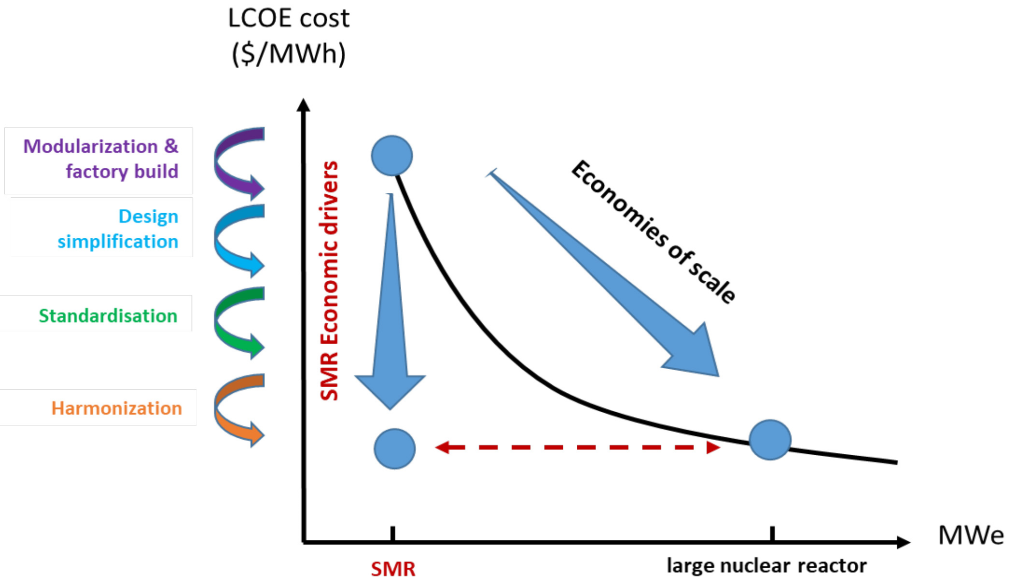
\includegraphics[width=0.8\textwidth]{content/figures/economy.png}
  \caption{Principales impulsores económicos para compensar las desventajas de la pequeña escala de los \acrshortpl{smr} (\cite{nea_smrs_2021}).}
  \label{fig:economy}
\end{figure}

Por último, vale la pena tener en mente los órdenes de magnitud del coste total de un \acrlong{smr}. Para ello, se emplean los resultados detallados a continuación de un estudio económico realizado por la \emph{Energy Policy Institute} de la Universidad de Chicago sobre el VOYGR-12 \acrshort{smr} de la empresa NuScale Power. 

\begin{table}[h]
  \centering
  \resizebox{0.7\textwidth}{!}{%
  \begin{tabular}{|c|c|}
  \hline
  \rowcolor[HTML]{ECF4FF} 
  \textbf{GENERAL DESCRIPTION}                      & \textbf{VOYGR-12 COSTS}  \\ \hline
  \rowcolor[HTML]{9698ED} 
  \textbf{Capitalized Direct Costs}                 & \textbf{\$1,805,616,142} \\ \hline
  \rowcolor[HTML]{CBCEFB} 
  Structures and Improvements                       & \$612,136,797            \\ \hline
  \rowcolor[HTML]{CBCEFB} 
  Reactor Plant Equipment                           & \$869,360,876            \\ \hline
  \rowcolor[HTML]{CBCEFB} 
  Turbine Plant Equipment                           & \$196,121,808            \\ \hline
  \rowcolor[HTML]{CBCEFB} 
  Electric Plant Equipment                          & \$34,982,052             \\ \hline
  \rowcolor[HTML]{CBCEFB} 
  Heat Rejection Systems                            & \$62,934,255             \\ \hline
  \rowcolor[HTML]{CBCEFB} 
  Miscellaneous Plant Equipment                     & \$30,080,354             \\ \hline
  \rowcolor[HTML]{FD6864} 
  \textbf{Capitalized Indirect Costs}               & \textbf{\$663,710,610}   \\ \hline
  \rowcolor[HTML]{FFCCC9} 
  Design Services at Home Office                    & \$130,978,572            \\ \hline
  \rowcolor[HTML]{FFCCC9} 
  Field Construction Management                     & \$60,906,859             \\ \hline
  \rowcolor[HTML]{FFCCC9} 
  Field Construction Supervision                    & \$246,930,385            \\ \hline
  \rowcolor[HTML]{FFCCC9} 
  Field Indirect Costs                              & \$224,894,794            \\ \hline
  \rowcolor[HTML]{FFCE93} 
  \textbf{Total Manufacture and Construction Costs} & \textbf{\$2,469,326,752} \\ \hline
  \end{tabular}%
  }
  \caption{Costes estimados de la fabricación y construcción del VOYGR-12 (\cite{cost_evaluation_nuscale}).}
  \label{tab:costes_voygr-12}
  \end{table}

  El VOYGR-12 \acrshort{smr} es una planta de 924 MWe constituida por 12 módulos de 77 MWe cada uno, por lo que el coste total por unidad de energía generada es de 2.672,43 \$/KWh. Por otro lado, el coste total estimado del reactor AP-1000 de Westinghouse ---con una potencia de 1.110 MWe--- es de \$6,8 mil millones (\cite{cost_ap1000}), resultando un coste total por unidad de energía producida de 6.126,13 \$/KWh, 2,3 veces superior que en el caso anterior. En la siguiente tabla se exponen los resultados recopilados, poniéndose de manifiesto la competitividad económica de los reactores modulares pequeños frente a los de gran escala:

  \begin{table}[h]
    \centering
    \resizebox{\textwidth}{!}{%
    \begin{tabular}{
    >{\columncolor[HTML]{FFCCC9}}c |
    >{\columncolor[HTML]{FFFFFF}}c |c|}
    \cline{2-3}
    \cellcolor[HTML]{FFFFFF}\textbf{} &
      \cellcolor[HTML]{ECF4FF}\textbf{AP-1000} &
      \cellcolor[HTML]{ECF4FF}\textbf{VOYGR-12 SMR} \\ \hline
    \multicolumn{1}{|c|}{\cellcolor[HTML]{FFCCC9}\textbf{Coste total estimado (\$)}} &
      6.800.000.000 &
      2.469.326.752 \\ \hline
    \multicolumn{1}{|c|}{\cellcolor[HTML]{FFCCC9}\textbf{Coste total por unidad de energía producida (\$/KWh)}} &
      6.126,13 &
      \cellcolor[HTML]{FFFFFF}2.672,43 \\ \hline
    \end{tabular}%
    }
    \caption{Comparación de costes entre una central nuclear de gran escala de generación III+ y un SMR en fase avanzada de desarrollo (\cite{cost_ap1000} y \cite{cost_evaluation_nuscale}).}
    \label{tab:comparacion_voygr_ap1000}
    \end{table}

\newpage

\subsubsection{Flexibilidad y diversidad de aplicaciones}

HABLAR AQUÍ DE LA PARTE "SOCIAL" DE LOS SMRs

APLICACIONES
Los SMR podrían apoyar la descarbonización de otros sectores energéticos, como la calefacción urbana, que requiere temperaturas de salida entre 80 y 200°C. Arabia Saudí también tiene interés en los SMR para cumplir sus necesidades de desalación del agua del mar.

Las temperaturas más altas proporcionadas por algunos SMR de IV Generación (450-850°C) puede servir para descarbonizar sectores industriales difíciles de sustituir hasta ahora, como refinado de petróleo, reformado con vapor para gas natural y producción de hidrógeno termoquímico.

Los SMR tienen características inherentes de seguimiento de carga que los hacen capaces de realizar una operación flexible en redes con una gran penetración de energías renovables variables, como eólica y solar fotovoltaica.

Los SMR se pueden implementar en áreas remotas y aisladas que no están conectadas a la red, en regiones con pequeñas redes eléctricas o en regiones con sitios adecuados limitados para grandes instalaciones nucleares.

En la Hoja de ruta de los SMR canadienses de 2018 se identificaron varias comunidades remotas fuera de la red e instalaciones mineras, donde los SMR podrían ser rentables como reemplazo de generadores diésel.

Flexibilidad mejorada: al aprovechar las capacidades de maniobrabilidad de los reactores existentes de la Generación II (NEA, 2012), los SMRs podrían lograr modos de seguimiento de carga mejorados resultantes de características de diseño inherentes, así como a través de la optimización de la operación de unidades multinúcleo (Ingersoll et al., 2015). Más generalmente, la flexibilidad de los SMRs también cubre las capacidades de despliegue (por ejemplo, menores requisitos de ubicación).

\newpage

\subsection{Clasificación de los Small Modular Reactors}

Pese a que existen diversos criterios para determinar los distintos tipos de \acrshortpl{smr}, en el presente proyecto se ha escogido la clasificación realizada por el \acrshort{oiea}, en la que se distinguen 6 grupos, de los cuales se ofrece a continuación una descripción y las tecnologías concretas desarrolladas:

\subsubsection{SMRs refrigerados por agua establecidos en tierra}

 Utilizan varias configuraciones de reactores de agua ligera (del inglés, \acrshortpl{lwr}) y de reactores de agua pesada (del inglés, \acrshortpl{hwr}) para establecerse en tierra y con posibilidad de aplicaciones sin conexión a la red. Se trata de la tecnología de \acrshort{smr} más madura en la actualidad, ya que la mayoría de las centrales nucleares de gran potencia en operación actualmente también son refrigeradas por agua.

 \begin{table}[h]
  \resizebox{\textwidth}{!}{%
  \begin{tabular}{|
  >{\columncolor[HTML]{FFCCC9}}c |c|c|c|c|c|}
  \hline
  \cellcolor[HTML]{ECF4FF}\textbf{Diseño} &
    \cellcolor[HTML]{ECF4FF}\textbf{Potencia (MWe)} &
    \cellcolor[HTML]{ECF4FF}\textbf{Tipo} &
    \cellcolor[HTML]{ECF4FF}\textbf{Diseñador} &
    \cellcolor[HTML]{ECF4FF}\textbf{País} &
    \cellcolor[HTML]{ECF4FF}\textbf{Estado} \\ \hline
  CAREM &
    30 &
    PWR &
    CNEA &
    Argentina &
    En construcción \\ \hline
  ACP100 &
    125 &
    PWR &
    CNNC/NPIC &
    China &
    En construcción \\ \hline
  CANDU SMR$^{TM}$ &
    300 &
    PHWR &
    Candu Energy &
    Canadá &
    Diseño conceptual \\ \hline
  CAP200 &
    \textgreater 200 &
    PWR &
    SPIC/SNERDI &
    China &
    Diseño básico \\ \hline
  DHR400 &
    400 MWt &
    PWR &
    CNNC &
    China &
    Diseño básico \\ \hline
  HAPPY200 &
    200 MWt &
    PWR &
    SPIC &
    China &
    Diseño detallado \\ \hline
  NHR200-II &
    200 MWt &
    PWR &
    Tsinghua University &
    China &
    Diseño básico \\ \hline
  TEPLATOR$^{TM}$ &
    \textless 150 MWt &
    HWR &
    \begin{tabular}[c]{@{}c@{}}UWB Pilsen \\ \& CIIRC CTU\end{tabular} &
    República checa &
    Diseño conceptual \\ \hline
  NUWARD$^{TM}$ &
    2 × 170 &
    PWR &
    EDF &
    Francia &
    Diseño conceptual \\ \hline
  IMR &
    350 &
    PWR &
    MHI &
    Japón &
    \begin{tabular}[c]{@{}c@{}}Diseño conceptual\\ completado\end{tabular} \\ \hline
  i-SMR &
    170 &
    PWR &
    \begin{tabular}[c]{@{}c@{}}KHNP \&\\ KAERI\end{tabular} &
    República de Corea &
    Diseño conceptual \\ \hline
  SMART &
    107 &
    PWR &
    \begin{tabular}[c]{@{}c@{}}KAERI \\ \& K.A.CARE\end{tabular} &
    \begin{tabular}[c]{@{}c@{}}República de Corea\\ y Arabia Saudí\end{tabular} &
    Diseño detallado \\ \hline
  RITM-200N &
    55 &
    PWR &
    \begin{tabular}[c]{@{}c@{}}JSC Afrikantov\\ \& OKBM Rosatom\end{tabular} &
    Rusia &
    \begin{tabular}[c]{@{}c@{}}Diseño detallado\\ completado\end{tabular} \\ \hline
  VK-300 &
    250 &
    BWR &
    NIKIET &
    Rusia &
    Diseño detallado \\ \hline
  KARAT-45 &
    45 – 50 &
    BWR &
    NIKIET &
    Rusia &
    Diseño conceptual \\ \hline
  KARAT-100 &
    100 &
    BWR &
    NIKIET &
    Rusia &
    Diseño conceptual \\ \hline
  RUTA-70 &
    70 MWt &
    PWR &
    NIKIET &
    Rusia &
    Diseño conceptual \\ \hline
  STAR &
    10 &
    PWR &
    STAR ENERGY &
    Suiza &
    Diseño básico \\ \hline
  Rolls-Royce SMR &
    470 &
    PWR &
    Rolls-Royce &
    Reino Unido &
    Diseño detallado \\ \hline
  VOYGR$^{TM}$ &
    4/6/12 × 77 &
    PWR &
    NuScale Power &
    EEUU &
    \begin{tabular}[c]{@{}c@{}}Fabricación de\\ equipos en proceso\end{tabular} \\ \hline
  BWRX-300 &
    270 – 290 &
    BWR &
    Hitachi &
    EEUU y Japón &
    Diseño detallado \\ \hline
  SMR-160 &
    160 &
    PWR &
    Holtec International &
    EEUU &
    \begin{tabular}[c]{@{}c@{}}Diseño preliminar\\ completado\end{tabular} \\ \hline
  Westinghouse SMR &
    \textgreater 225 &
    PWR &
    Westinghouse &
    EEUU &
    \begin{tabular}[c]{@{}c@{}}Diseño conceptual\\ completado\end{tabular} \\ \hline
  mPower &
    2 × 195 &
    PWR &
    BWX Technologies &
    EEUU &
    Diseño conceptual \\ \hline
  OPEN20 &
    22 &
    PWR &
    Last Energy &
    EEUU &
    Diseño detallado \\ \hline
  \end{tabular}%
  }
  \caption{Diseños existentes de SMRs refrigerados por agua establecidos en tierra (\cite{iaea_smr_booklet_2022}).}
  \label{tab:smrs_agua_tierra}
  \end{table}

\subsubsection{SMRs refrigerados por agua establecidos en el mar}

Instalaciones flotantes montadas en barcos o sumergidas bajo el mar. Ofrecen una gran versatilidad gracias a su capacidad de desplazamiento. A este grupo pertenecen los dos reactores KLT-40S pertenecientes a la \textbf{planta de energía nuclear flotante Akademik Lomonosov}, que comenzó su operación comercial en Pevek (Rusia) en mayo de 2020, siendo \textbf{el primer diseño de SMR conectado a la red}, con una potencia eléctrica total ---entre ambos reactores--- de 70 MWe y 300 MWt, proporcionando así electricidad a una ciudad de 100.000 habitantes.

\begin{figure}[h]
    \centering
    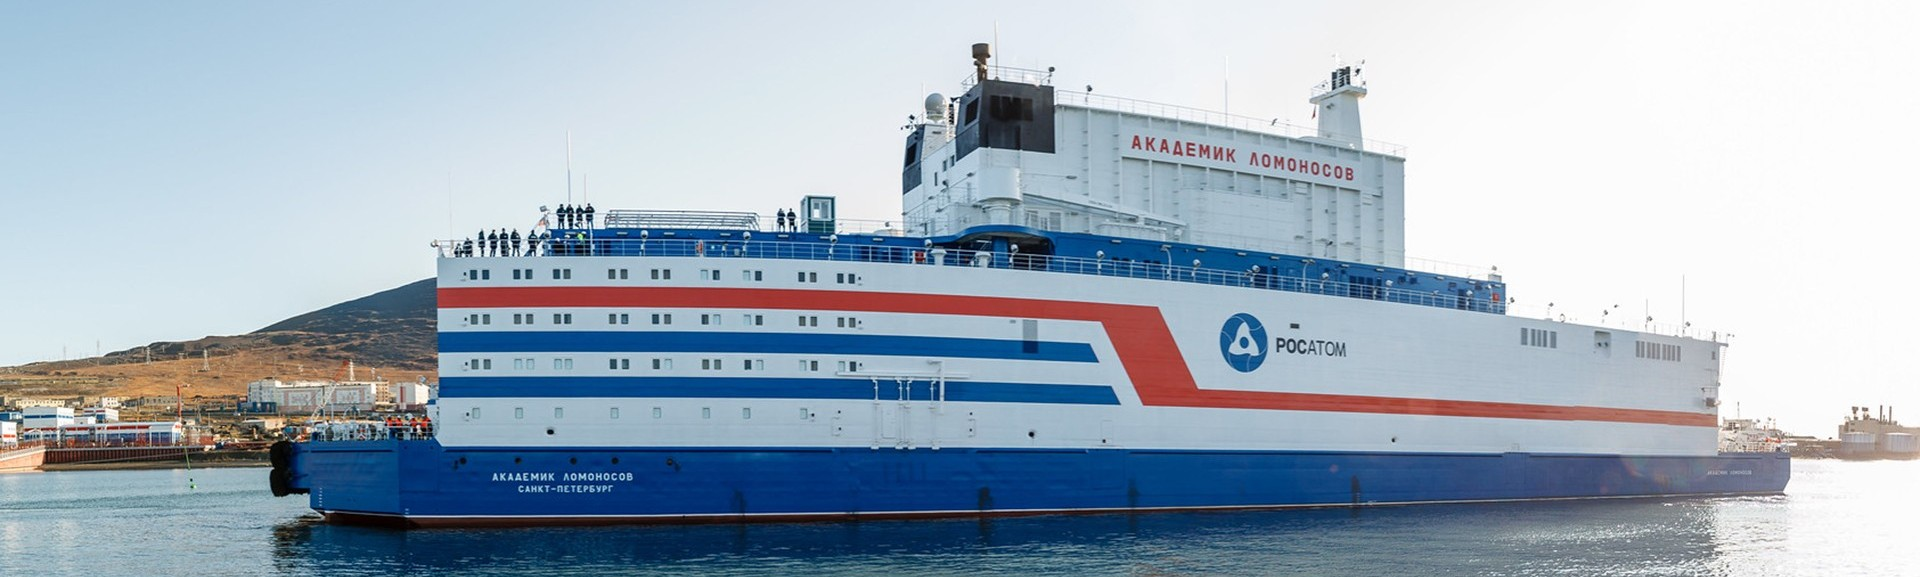
\includegraphics[width=0.8\textwidth]{content/figures/akademik_lomonosov.jpg}
    \caption{La central nuclear flotante Akademik Lomonosov (\cite{nuclear_españa}).}
    \label{fig:akademik_lomonosov}
\end{figure}

\begin{table}[h]
  \resizebox{\textwidth}{!}{%
  \begin{tabular}{|
  >{\columncolor[HTML]{FFCCC9}}c |c|c|c|c|c|}
  \hline
  \cellcolor[HTML]{ECF4FF}\textbf{Diseño} &
    \cellcolor[HTML]{ECF4FF}\textbf{Potencia (MWe)} &
    \cellcolor[HTML]{ECF4FF}\textbf{Tipo} &
    \cellcolor[HTML]{ECF4FF}\textbf{Diseñador} &
    \cellcolor[HTML]{ECF4FF}\textbf{País} &
    \cellcolor[HTML]{ECF4FF}\textbf{Estado} \\ \hline
  KLT-40S &
    2 × 35 &
    PWR &
    JSC Afrikantov OKBM &
    Rusia &
    En operación \\ \hline
  ACPR50S &
    50 &
    PWR &
    CGNPC &
    China &
    Diseño detallado \\ \hline
  ACP100S &
    125 &
    PWR &
    CNNC/NPIC &
    China &
    Diseño básico \\ \hline
  BANDI-60 &
    60 &
    PWR &
    KEPCO E\&C &
    Corea del Sur &
    Diseño conceptual \\ \hline
  ABV-6E &
    6 – 9 &
    PWR &
    \begin{tabular}[c]{@{}c@{}}JSC Afrikantov\\ OKBM, Rosatom\end{tabular} &
    Rusia &
    Diseño final \\ \hline
  RITM-200M &
    50 &
    PWR &
    \begin{tabular}[c]{@{}c@{}}JSC Afrikantov\\ OKBM, Rosatom\end{tabular} &
    Rusia &
    \begin{tabular}[c]{@{}c@{}}Diseño básico\\ completado\end{tabular} \\ \hline
  VBER-300 &
    325 &
    PWR &
    \begin{tabular}[c]{@{}c@{}}JSC Afrikantov\\ OKBM, Rosatom\end{tabular} &
    Rusia &
    \begin{tabular}[c]{@{}c@{}}Fase de \\ licenciamiento\end{tabular} \\ \hline
  SHELF-M &
    \textgreater \space 10 &
    PWR &
    NIKIET &
    Rusia &
    Diseño básico \\ \hline
  \end{tabular}%
  }
  \caption{Diseños existentes de SMRs refrigerados por agua establecidos en el mar (\cite{iaea_smr_booklet_2022}).}
  \label{tab:smrs_agua_mar}
  \end{table}

\subsubsection{SMRs refrigerados por gas de alta temperatura (del inglés, HTGR)}

Reactores de \acrshort{genIV} que proporcionan calor a elevada temperatura (superior a 750°C) y que pueden ser utilizados para generar electricidad de forma más eficiente y con una variedad de aplicaciones industriales. Dentro de esta categoría, hay múltiples diseños en desarrollo y alguno en operación, como el \textbf{HTR-PM de China, el primer \acrshort{htgr} en operación del mundo}. Con un reactor de lecho de bolas\footnote{Reactor de muy alta temperatura moderado con grafito y refrigerado por gas, cuyos elementos de combustible son esféricos (denominados ``bolas'') y contienen miles de partículas \acrshort{triso}. Estos combustibles tri-isotrópicos constan de carburo de uranio revestido con varias capas de carbón pirolítico y dióxido de silicio para retener los productos de fisión a altas temperaturas.}, una potencia eléctrica de 210 MWe y una potencia térmica de 500 MWt, se conectó a la red en diciembre de 2021 y comenzó a operar comercialmente a plena potencia en diciembre de 2023, con el objetivo de reemplazar las centrales de carbón presentes en el interior de China. También se incluyen en este grupo tres reactores de prueba \acrshort{htgr}, dos de los cuales han estado en operación durante más de veinte años para realizar pruebas en Japón y China.

\begin{figure}[h]
  \centering
  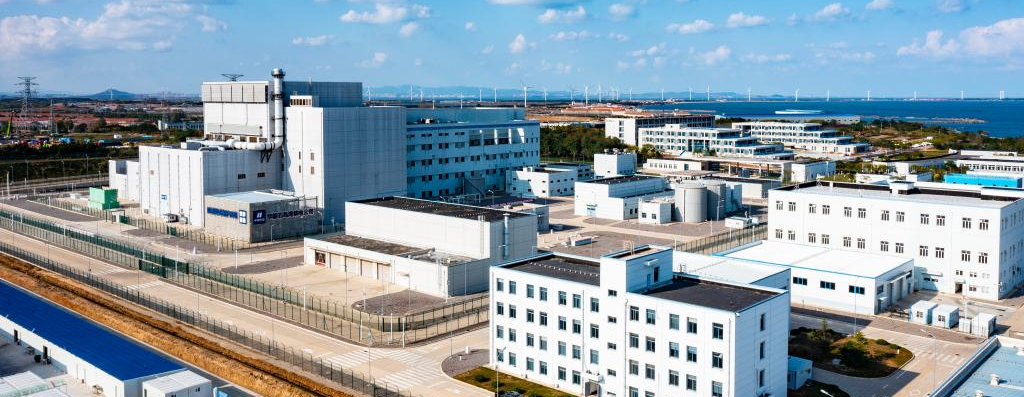
\includegraphics[width=0.65\textwidth]{content/figures/HTR_PM_china.jpg}
  \caption{Primer reactor de \acrshort{genIV} en operación: HTR-PM de China (\cite{htr_pm_china}).}
  \label{fig:htr_pm_china}
\end{figure}

\begin{table}[h]
  \centering
  \resizebox{0.91\textwidth}{!}{%
  \begin{tabular}{|
  >{\columncolor[HTML]{FFCCC9}}c |c|c|c|c|c|}
  \hline
  \cellcolor[HTML]{ECF4FF}\textbf{Diseño} &
    \cellcolor[HTML]{ECF4FF}\textbf{Potencia (MWe)} &
    \cellcolor[HTML]{ECF4FF}\textbf{Tipo} &
    \cellcolor[HTML]{ECF4FF}\textbf{Diseñador} &
    \cellcolor[HTML]{ECF4FF}\textbf{País} &
    \cellcolor[HTML]{ECF4FF}\textbf{Estado} \\ \hline
  HTR-PM &
    210 &
    \begin{tabular}[c]{@{}c@{}}HTGR\\ (lecho de bolas)\end{tabular} &
    \begin{tabular}[c]{@{}c@{}}INET, Tsinghua\\ University\end{tabular} &
    China &
    En operación \\ \hline
  STARCORE &
    14/20/60 &
    \begin{tabular}[c]{@{}c@{}}HTGR\\ (prismático)\end{tabular} &
    StarCore Nuclear &
    Canadá &
    Diseño preconceptual \\ \hline
  JIMMY &
    \begin{tabular}[c]{@{}c@{}}10 – 20\\ MWt\end{tabular} &
    \begin{tabular}[c]{@{}c@{}}HTGR\\ (prismático)\end{tabular} &
    JIMMY ENERGY SAS &
    Francia &
    Diseño detallado \\ \hline
  GTHTR300 &
    100 – 300 &
    \begin{tabular}[c]{@{}c@{}}HTGR\\ (prismático)\end{tabular} &
    JAEA Consortium &
    Japón &
    Diseño básico \\ \hline
  GT-MHR &
    288 &
    \begin{tabular}[c]{@{}c@{}}HTGR\\ (prismático)\end{tabular} &
    JSC Afrikantov OKBM &
    Rusia &
    \begin{tabular}[c]{@{}c@{}}Diseño preliminar\\ completado\end{tabular} \\ \hline
  MHR-T &
    4 × 205,5 &
    HTGR &
    JSC Afrikantov OKBM &
    Rusia &
    Diseño conceptual \\ \hline
  MHR-100 &
    25 – 87 &
    HTGR &
    JSC Afrikantov OKBM &
    Rusia &
    Diseño conceptual \\ \hline
  AHTR-100 &
    50 &
    \begin{tabular}[c]{@{}c@{}}HTGR\\ (lecho de bolas)\end{tabular} &
    Eskom Holdings SOC &
    Sudáfrica &
    \begin{tabular}[c]{@{}c@{}}Diseño conceptual\\ completado\end{tabular} \\ \hline
  PBMR-400 &
    165 &
    \begin{tabular}[c]{@{}c@{}}HTGR\\ (lecho de bolas)\end{tabular} &
    PBMR SOC &
    Sudáfrica &
    \begin{tabular}[c]{@{}c@{}}Diseño preliminar\\ completado\end{tabular} \\ \hline
  HTMR100 &
    35 &
    \begin{tabular}[c]{@{}c@{}}HTGR\\ (lecho de bolas)\end{tabular} &
    STL Nuclear (Pty) &
    Sudáfrica &
    Diseño básico \\ \hline
  EM$^2$ &
    265 &
    GFR &
    General Atomics &
    EEUU &
    Diseño conceptual \\ \hline
  FMR &
    50 &
    GFR &
    General Atomics &
    EEUU &
    Diseño conceptual \\ \hline
  Xe-100 &
    82,5 &
    \begin{tabular}[c]{@{}c@{}}HTGR\\ (lecho de bolas)\end{tabular} &
    X-Energy LLC &
    EEUU &
    Diseño básico \\ \hline
  SC-HTGR &
    272 &
    \begin{tabular}[c]{@{}c@{}}HTGR\\ (prismático)\end{tabular} &
    Framatome &
    EEUU &
    Diseño preliminar \\ \hline
  PeLUIt / RDE &
    40 MWt &
    \begin{tabular}[c]{@{}c@{}}HTGR\\ (lecho de bolas)\end{tabular} &
    BRIN &
    Indonesia &
    Diseño conceptual \\ \hline
  HTR-10 &
    2,5 &
    \begin{tabular}[c]{@{}c@{}}HTGR\\ (lecho de bolas)\end{tabular} &
    \begin{tabular}[c]{@{}c@{}}INET, Tsinghua\\ University\end{tabular} &
    China &
    Operable \\ \hline
  HTTR &
    30 MWt &
    \begin{tabular}[c]{@{}c@{}}HTGR\\ (prismático)\end{tabular} &
    JAEA &
    Japón &
    En operación \\ \hline
  \end{tabular}%
  }
  \caption{Diseños existentes de SMRs refrigerados por gas de alta temperatura (\cite{iaea_smr_booklet_2022}).}
  \label{tab:smrs_gas_alta_temp}
  \end{table}

\newpage

\subsubsection{SMRs rápidos refrigerados por metal líquido (del inglés, LMFR)}

Los metales líquidos que utilizan como regrigerantes incluyen sodio, plomo puro y eutéctico de plomo-bismuto. Hay grandes avances en el desarrollo y despliegue de esta tecnología de \acrshortpl{lmfr}. Prueba de ello es el BREST-OD-300, un reactor de neutrones rápidos refrigerado por plomo que se está construyendo en Seversk (Rusia) y se planea su puesta en marcha en 2026. Se trata de un proyecto prototipo para futuros diseños que empleen un ciclo combustible nuclear cerrado, en el cual pueda reutilizarse el combustible gastado mediante la separación del uranio, plutonio y actínidos minoritarios (Np, Am y Cm), para ser transmutados en estos reactores rápidos (\cite{apuntes_centrales}).

\begin{table}[h]
  \resizebox{\textwidth}{!}{%
  \begin{tabular}{|
  >{\columncolor[HTML]{FFCCC9}}c |c|c|c|c|c|}
  \hline
  \cellcolor[HTML]{ECF4FF}\textbf{Diseño} &
    \cellcolor[HTML]{ECF4FF}\textbf{Potencia (MWe)} &
    \cellcolor[HTML]{ECF4FF}\textbf{Tipo} &
    \cellcolor[HTML]{ECF4FF}\textbf{Diseñador} &
    \cellcolor[HTML]{ECF4FF}\textbf{País} &
    \cellcolor[HTML]{ECF4FF}\textbf{Estado} \\ \hline
  BREST-OD-300 &
    300 &
    LMFR &
    NIKIET &
    Rusia &
    En construcción \\ \hline
  ARC-100 &
    100 &
    LMFR &
    ARC Clean Energy &
    Canadá &
    Diseño preliminar \\ \hline
  4S &
    10 &
    LMFR &
    \begin{tabular}[c]{@{}c@{}}Toshiba Energy\\ Systems \&\\ Solutions Corporation\end{tabular} &
    Japón &
    Diseño detallado \\ \hline
  MicroURANUS &
    20 &
    LBE-cooled Reactor &
    UNIST &
    Corea del Sur &
    Diseño conceptual \\ \hline
  LFR-AS-200 &
    200 &
    LMFR &
    newcleo srl &
    Italia &
    Diseño conceptual \\ \hline
  SVBR &
    100 &
    LMFR &
    \begin{tabular}[c]{@{}c@{}}JSC AKME\\ Engineering\end{tabular} &
    Rusia &
    Diseño detallado \\ \hline
  SEALER-55 &
    55 &
    LMFR &
    LeadCold &
    Suiza &
    Diseño conceptual \\ \hline
  Westinghouse LFR &
    450 &
    LMFR &
    Westinghouse &
    EEUU &
    Diseño conceptual \\ \hline
  \end{tabular}%
  }
  \caption{Diseños existentes de SMRs rápidos refrigerados por metal líquido (\cite{iaea_smr_booklet_2022}).}
  \label{tab:smrs_metal_liquido_rapidos}
  \end{table}

\subsubsection{SMRs de sales fundidas (del inglés, MSR)}

Reactores de \acrshort{genIV} alimentados y refrigerados por sales fundidas, propiedad que les confiere múltiples ventajas, incluida una seguridad mejorada debido a la propiedades de las sales, un sistema de refrirefrigeración de fase única a baja presión que elimina la necesidad de un gran contenedor, un sistema de alta temperatura con gran eficiencia y un ciclo de combustible flexible. Se están llevando a cabo actividades preliminares de licenciamiento con varios de estos diseños de \acrshortpl{msr} con reguladores de Canadá, Dinamarca, Países Bajos, Reino Unido y los Estados Unidos.

\begin{table}[h]
  \resizebox{\textwidth}{!}{%
  \begin{tabular}{|
  >{\columncolor[HTML]{FFCCC9}}c |c|c|c|c|c|}
  \hline
  \cellcolor[HTML]{ECF4FF}\textbf{Diseño} &
    \cellcolor[HTML]{ECF4FF}\textbf{Potencia (MWe)} &
    \cellcolor[HTML]{ECF4FF}\textbf{Tipo} &
    \cellcolor[HTML]{ECF4FF}\textbf{Diseñador} &
    \cellcolor[HTML]{ECF4FF}\textbf{País} &
    \cellcolor[HTML]{ECF4FF}\textbf{Estado} \\ \hline
  IMSR400 &
    2 × 195 &
    MSR &
    Terrestrial Energy &
    Canadá &
    Diseño detallado \\ \hline
  SSR-W &
    300 &
    MSR &
    Moltex Energy &
    Canadá &
    Diseño conceptual \\ \hline
  smTMSR-400 &
    168 &
    MSR &
    CAS/SINAP &
    China &
    Diseño pre-conceptual \\ \hline
  CMSR &
    100 &
    MSR &
    \begin{tabular}[c]{@{}c@{}}Seaborg Technologies\\ ApS\end{tabular} &
    Dinamarca &
    Diseño conceptual \\ \hline
  \begin{tabular}[c]{@{}c@{}}Copenhagen Atomics\\ Waste Burner\end{tabular} &
    20 MWt &
    MSR &
    Copenhagen Atomics &
    Dinamarca &
    Diseño detallado \\ \hline
  FUJI &
    200 &
    MSR &
    ITMSF &
    Japón &
    \begin{tabular}[c]{@{}c@{}}Diseño preliminar\\ completado\end{tabular} \\ \hline
  THORIZON &
    40 – 120 &
    MSR &
    THORIZON &
    Holanda &
    Diseño conceptual \\ \hline
  SSR-U &
    16 &
    MSR &
    Moltex Energy &
    Reino Unido &
    Diseño básico \\ \hline
  KP-FHR &
    140 &
    FHR &
    KAIROS Power &
    EEUU &
    Diseño conceptual \\ \hline
  Mk1 PB-FHR &
    100 &
    FHR &
    UC Berkeley &
    EEUU &
    Diseño pre-conceptual \\ \hline
  MCSFR &
    \begin{tabular}[c]{@{}c@{}}50 / 200 /\\ 400 / 1200\end{tabular} &
    MSR &
    Elysium Industries &
    EEUU &
    Diseño conceptual \\ \hline
  LFTR &
    250 &
    MSR &
    Flibe Energy &
    EEUU &
    Diseño conceptual \\ \hline
  ThorCon &
    250 &
    MSR &
    ThorCon International &
    \begin{tabular}[c]{@{}c@{}}EEUU\\ e Indonesia\end{tabular} &
    \begin{tabular}[c]{@{}c@{}}Diseño preliminar\\ completado\end{tabular} \\ \hline
  \end{tabular}%
  }
  \caption{Diseños existentes de SMRs de sales fundidas (\cite{iaea_smr_booklet_2022}).}
  \label{tab:smrs_sales_fundidas}
  \end{table}

\subsubsection{Microreactores modulares (del inglés, MMR)}

Diseños de \textbf{menos de 10 MWe de potencia}, con capacidad de opearción semi-autónoma y con una mejor transportabilidad que los \acrshortpl{smr} más grandes. Existen varios diseños punteros tecnológicamente ---incluidos de \acrshort{genIV}---, en los que el reactor utiliza diversos refrigerantes en cada caso: agua ligera, helio, sales fundidas o metal líquido. Los \acrshortpl{mmr} son especialmente adecuados para operar fuera de la red en ubicaciones remotas, en situaciones de necesidad de abastecimiento de emergencia en hospitales o comunidades afectadas por desastres naturales, para desalinizar agua del mar, etc. Estos microrreactores se encuentran en las primeras fases de desarrollo y, en las aplicaciones concretas anteriormente expuestas, se espera que sean muy competitivos frente a las fuentes de electricidad previamente utilizadas.

\begin{figure}[h]
    \centering
    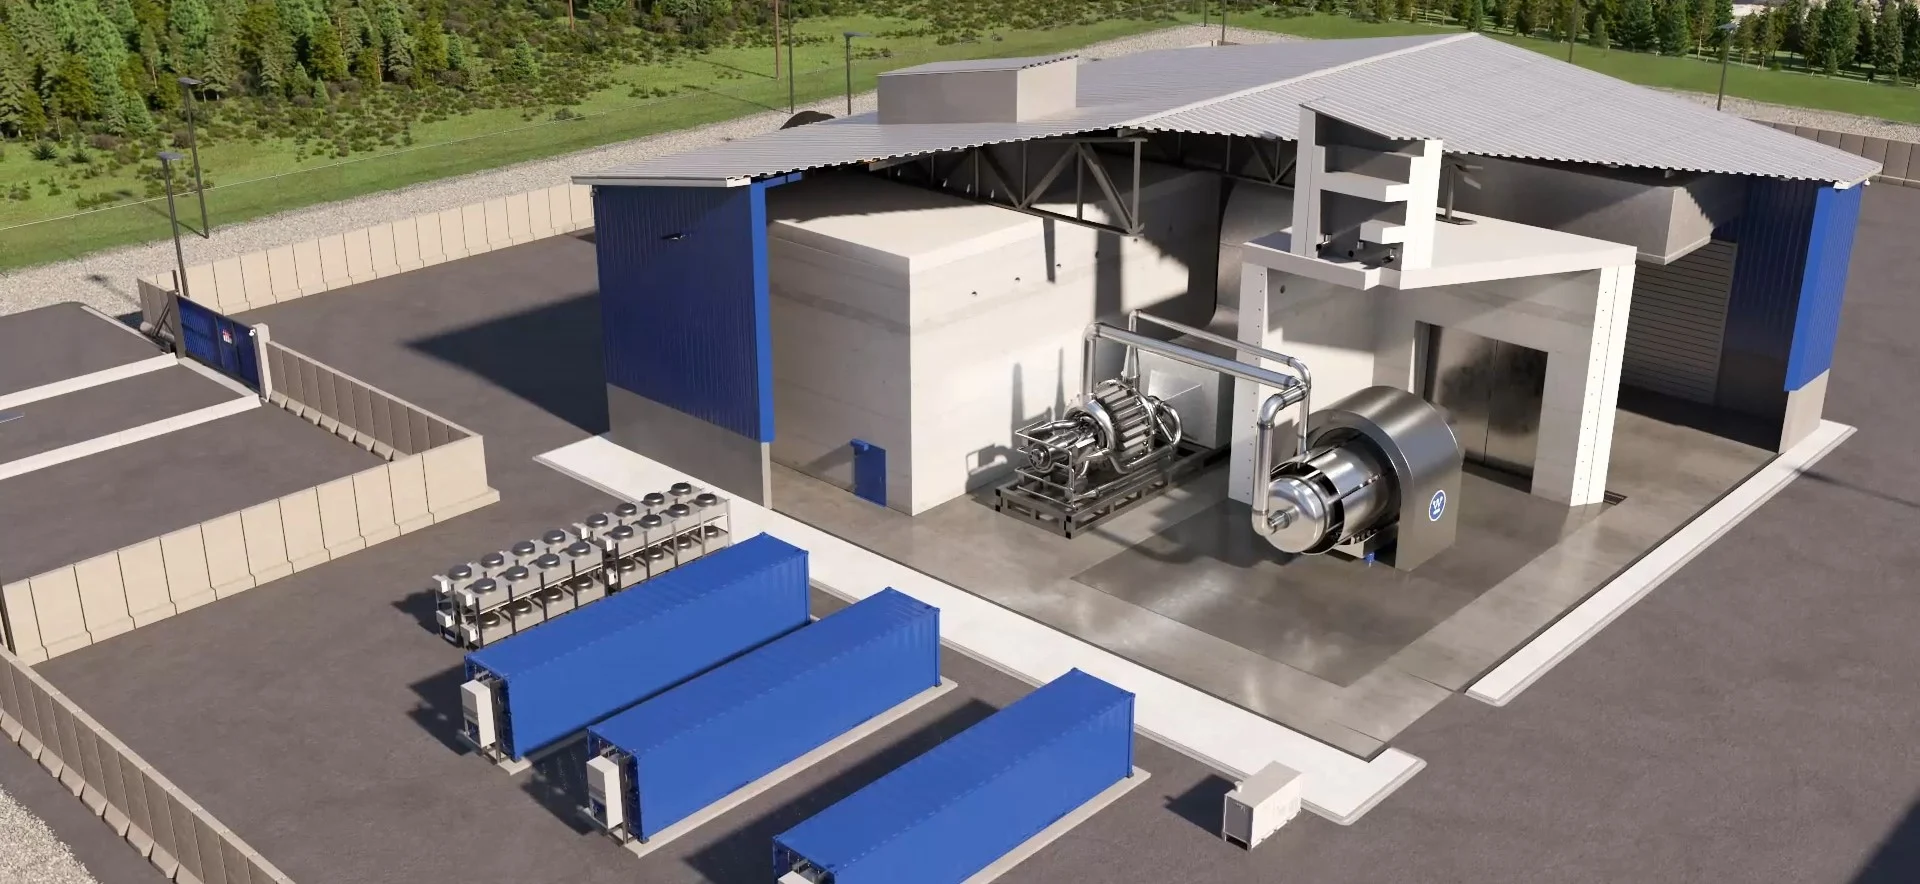
\includegraphics[width=0.7\textwidth]{content/figures/evinci.jpg}
    \caption{Render del \emph{eVinci$^{TM}$ Microreactor} de Westinghouse, con una potencia de 5 MWe y 13 MWt (\cite{evinci}).}
    \label{fig:evinci}
\end{figure}

\begin{table}[]
  \resizebox{\textwidth}{!}{%
  \begin{tabular}{|
  >{\columncolor[HTML]{FFCCC9}}c |c|c|c|c|c|}
  \hline
  \cellcolor[HTML]{ECF4FF}\textbf{Diseño} &
    \cellcolor[HTML]{ECF4FF}\textbf{Potencia (MWe)} &
    \cellcolor[HTML]{ECF4FF}\textbf{Tipo} &
    \cellcolor[HTML]{ECF4FF}\textbf{Diseñador} &
    \cellcolor[HTML]{ECF4FF}\textbf{País} &
    \cellcolor[HTML]{ECF4FF}\textbf{Estado} \\ \hline
  Energy Well & 8        & FHTR & Centrum výzkumu Řež & República Checa & Diseño pre-conceptual \\ \hline
  MoveluX &
    3 – 4 &
    \begin{tabular}[c]{@{}c@{}}Tubos de\\ disipación de calor\end{tabular} &
    \begin{tabular}[c]{@{}c@{}}Toshiba Energy\\ Systems \& Solutions\\ Corporation\end{tabular} &
    Japón &
    Diseño conceptual \\ \hline
  ELENA &
    0,068 &
    PWR &
    \begin{tabular}[c]{@{}c@{}}National Research\\ Centre\\ “Kurchatov Institute”\end{tabular} &
    Rusia &
    Diseño conceptual \\ \hline
  UNITHERM    & 6,6      & PWR  & NIKIET              & Rusia           & Diseño conceptual     \\ \hline
  AMR         & 3        & HTGR & STL Nuclear (Pty)   & Sudáfrica       & Diseño pre-conceptual \\ \hline
  LFR-TL-30   & 30       & LMFR & newcleo             & Reino Unido     & Diseño conceptual     \\ \hline
  U-Battery   & 4        & HTGR & Urenco              & Reino Unido     & Diseño conceptual     \\ \hline
  Aurora      & 1,5 – 50 & LMFR & OKLO                & EEUU            & Diseño detallado      \\ \hline
  HOLOS-QUAD  & 10       & HTGR & HolosGen LLC        & EEUU            & Diseño detallado      \\ \hline
  MARVEL &
    0,015 – 0,027 &
    LMFR &
    \begin{tabular}[c]{@{}c@{}}Idaho National\\ Laboratory\end{tabular} &
    EEUU &
    \begin{tabular}[c]{@{}c@{}}Fabricación de equipos\\ en proceso\end{tabular} \\ \hline
  MMR$^{TM}$ &
    \textgreater 5 y \textgreater 10 &
    HTGR &
    \begin{tabular}[c]{@{}c@{}}Ultra Safe Nuclear\\ Corporation\end{tabular} &
    EEUU &
    Diseño básico \\ \hline
  \begin{tabular}[c]{@{}c@{}}Westinghouse\\ eVinci$^{TM}$\end{tabular} &
    2 – 3,5 &
    \begin{tabular}[c]{@{}c@{}}Tubos de\\ disipación de calor\end{tabular} &
    Westinghouse &
    EEUU &
    \begin{tabular}[c]{@{}c@{}}Diseño conceptual\\ completado\end{tabular} \\ \hline
  \end{tabular}%
  }
  \caption{Diseños existentes de MMRs (\cite{iaea_smr_booklet_2022}).}
  \label{tab:mmrs}
  \end{table}

\subsection{El reactor AP300}

Pendiente\dots

\subsection{NuScale Power}

Pendiente\dots